\section{Śledzenie promieni}

\subsection{Podstawowy algorytm śledzenia promieni}

Metoda śledzenia promieni pozwala określić widoczność obiektów znajdujących
się na scenie (a tym samym na generowanie obrazu) na zasadzie śledzenia umownych promieni świetlnych biegnących od obserwatora w scenę. W perspektywicznym rozumieniu sceny (a takiego dotyczy algorytm zaimplementowany na potrzeby tej pracy), pierwszym krokiem algorytmu jest wybranie środka rzutowania (nazywanego okiem obserwatora) oraz rzutni (powierzchnia na której zostanie odwzorowana trójwymiarowa scena). Rzutnię (a właściwie interesujący nas wycinek rzutni - abstrakcyjne okno obserwatora) można podzielić na regularną siatkę, w której każde pole odpowiada jednemu pikselowi ekranie urządzenia (tzw. układ urządzenia). Kolejnym krokiem algorytmu jest wypuszczenie promienia wychodzącego z oka obserwatora, przechodzącego przez dany piksel ekranu i lecącego dalej - w scenę. Kolor piksela jest ustalany na podstawie barwy i oświetlenia najbliższego obiektu (więcej o metodach oświetlenia można przeczytać w rozdziale !TU WSTAW ROZDZIAŁ!), który został przecięty przez wysłany promień. W przypadku braku kolizji piksel przybiera barwę otoczenia. 

\begin{figure}[h!]
\centering
  \caption{Rzut perspektywiczny, źródło: http://www.zsk.ict.pwr.wroc.pl}
  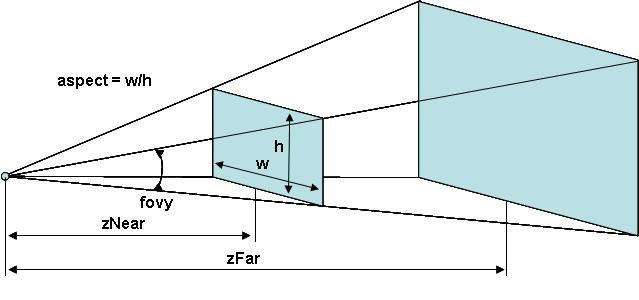
\includegraphics[width=10cm]{perspective_view.jpg}
\end{figure}

Poniżej przedstawiono pseudokod podstawowego śledzenia promieni

\begin{algorithmic}
\\
piksele, obiekty
\State obj = null
\State dist = max
\\
\State wybór środka rzutowania i rzutni
\\
\For{piksel in piksele}
	 \State wyznacz promień
	 \For{obiekt in obiekty}
	 \If {promień przecina obiekt i dystans $<$ dist}
    		\State obj = obiekt
    		\State dist = dystans
     \EndIf
	 \EndFor
\EndFor
\\
\State ustal kolor piksela na podstawie obj
\\
\end{algorithmic}

Więcej na temat podstaw śledzenia promieni można przeczytać w \cite{foley95, suffern2007, scratch}

\subsubsection{Obliczenie przecięć}

Kluczowym elementem metody śledzenia promieni jest obliczanie przecięć promieni z obiektami sceny - zajmuje one znakomitą większość czasu generowania sceny \cite{suffern2007}. W związku z tym, chcąc optymalizować działanie programu największy wysiłek wkłada się w dwa poniższe elementy:

\begin{enumerate}

\item Zmniejszenie kosztu wyznaczenia punktu przecięcia promienia z obiektem (stosowanie optymalnych czasowo algorytmów badania przecięcia)

\item Zmniejszenie liczby obiektów, dla których należy zbadać, czy dany promień je przecina (np. poprzez zastosowanie metody brył otaczających, czy wprowadzenie hierarchii sceny)

\end{enumerate}

Wyznaczenie przecięcia promienia z obiektem polega na rozwiązaniu szeregu układu równań zależnych od tego, z jakim obiektem szukamy przecięcia. Najczęściej scena składa się z wielu różnych wielokątów (poligonów), które w połączeniu ze sobą tworzą tzw. siatkę trójwymiarową (ang. mesh) reprezentującą dany obiekt - takie rozwiązanie daje możliwość tworzenia rozmaitych i skomplikowanych modeli 3D (podstawową składową takiego modelu nazywamy prymitywem). Najczęstszym rodzajem wykorzystywanych prymitywów (w grafice 3D) są trójkąty, gdyż da się z nich ułożyć dowolny inny wielokąt. Innym typem obiektów, z jakimi możemy szukać przecięcia, są wszelkiego rodzaju bryły dające zapisać się raczej w postaci prostego równania, niż zbioru punktów. Popularnym, w śledzeniu promieni, przykładem takiej bryły jest kula, lub torus. Poniżej przedstawiono metody badania przecięcia promieni z obiektami, które będą wykorzystywane w programie. Dokładny opis algorytmów oraz ich przykładową implementację można znaleźć w między innymi w \cite{dunn02, scratch}.

\paragraph{Przecięcie promienia z kulą}
Dane są równania promienia i kuli mające następującą postać:
\\
$p = p_0 + tv$ \\
$(x - x_s)^2 + (y - y_s)^2 + (z - z_s)^2 - r^2 = 0$ \\
\\
gdzie
\\
$p_0$ - punkt początkowy promienia $(x_0, y_0, z_0)$ \\
$v$ - wektor kierunkowy promienia o długości 1 $(x_v, y_v, z_v)$ \\
$t$ - parametr określający odległość danego punktu, należącego do promienia, od jego początku tego promienia \\
$(x_s, y_s, z_s)$ - współrzędne środka kuli \\
$r$ - promień kuli \\
\\
Po podstawieniu równania promienia do równania kuli otrzymujemy równianie kwadratowe zależne od współczynnika t:
\\
$a = x_v^2 + y_v^2 + z_v^2 = 1$ \\
$b = x_v(x_0 - x_s) + y_v(y_0 - y_s) + z_v(z_0 - z_s)$ \\
$c = (x_0 - x_s)^2 + (y_0 - y_s)^2 + (z_0 - z_s)^2 - r^2$ \\
\\
Jeżeli istnieją rozwiązania ($\Delta \geq 0$) to $t_{1,2} = -b \pm \sqrt{\Delta}$. Najczęściej interesują nas tylko rozwiązania dodatnie (dla $t < 0$ przecięcie znajduje się za promieniem). W przypadku dwóch rozwiązań dodatnich wybieramy to mniejsze (bliższy punkt przecięcia). Podstawiając rozwiązanie do równania promienia otrzymamy punkt przecięcia zawierający w powierzchni kuli.

\paragraph{Przecięcie promienia z płaszczyzną}

Płaszczyzna nie jest prymitywem, gdyż z definicji jest ona nieskończona, jednak wyliczenie przecięcia promienia z płaszczyzną jest najczęściej pierwszym krokiem znalezienia przecięcia z dowolnym poligonem (najpierw znajduje się przecięcie z płaszczyzną wyznaczoną przez dany wielokąt, a sprawdza się, czy punkt przecięcia się w nim zawiera). Dodatkowo algorytm przecięcia promienia z płaszczyzną jest wykorzystywany w tworzeniu drzewa BSP (o którym można dowiedzieć się więcej w rozdziale !TU WSTAW ROZDZIAŁ!. \\

Dane są równanie promienia i równanie płaszczyzny: \\
$p = p_0 + tv$ \\
$Ax + By + Cz + D = P \bullet N + D = 0$ \\
\\
gdzie
\\
$p_0$ - punkt początkowy promienia $(x_0, y_0, z_0)$ \\
$v$ - wektor kierunkowy promienia o długości 1 $(x_v, y_v, z_v)$ \\
$t$ - parametr określający odległość danego punktu, należącego do promienia, od jego początku tego promienia \\
$P$ - dowolny punkt płaszczyzny \\
$N$ - wektor normalny do płaszczyzny \\
\\
Podstawiając równanie promienia (dowolny punkt promienia) za punkt płaszczyzny otrzymujemy: \\
\\
$(p_0 + tv) \bullet N + D = 0$ \\
$t = -(p_0 \bullet N + D)/(v \bullet N)$ \\
\\
Podstawiając $t$ do równania promienia otrzymujemy punkt przecięcia. Jeżeli $t < 0$ to płaszczyzna znajduje się za promieniem, w przeciwnym przypadku przed (gdy $t = 0$ punkt początkowy zawiera się w płaszczyźnie). Należy zwrócić uwagę, że $v \bullet N$ nie może być równe zero - jeżeli jest, znaczy to że promień nigdy nie przecina płaszczyzny (jest do niej równoległy).

\paragraph{Przecięcie promienia z trójkątem}

Poniżej przedstawiono dwa sposoby na znalezienie punktu przecięcia promienia z trójkątem (trójkąt jest zdefiniowany poprzez trzy znane punkty - a, b, c).

\subparagraph{Algorytm klasyczny}

1. Wyznaczenie równania płaszczyzny z trójkąta:

a) Obliczenie wektora normalnego do trójkąta:

	$v = (b - a) \times (c - a)$
	$n = v/|v|$

b) Wyznaczenie płaszczyzny poprzez podstawienie do równania ogólnego  dowolnego punktu będącego kątem trójkąta i wektora normalnego.

2. Znalezienie punktu przecięcia płaszczyzny z promieniem - punkt ten nazwijmy $x$.

3. Sprawdzenie, czy punkt przecięcia z płaszczyzną leży wewnątrz trójkąta:

Punkt leży wewnątrz trójkąta, jeżeli znajduje po tej samej stronie każdej krawędzi, co punkt nie należący do tej krawędzi:

$(b - a) \times (x - a) \bullet n > 0$
$(c - b) \times (x - b) \bullet n > 0$
$(a - c) \times (x - c) \bullet n > 0$

\subparagraph{Algorytm Möller – Trumbore}

Algorytm ,,Möller – Trumbore'' nazwany tak na cześć swoich twórców - Tomasa Möllera and Bena Trumbore'a - jest tzw. szybkim algorytmem badania przecięcia się promienia z trójkątem bez potrzeby wyznaczania płaszczyzny, na której leży trójkąt. Algorytm ten wykorzystuje współrzędne barycentryczne. Najpierw wybieramy dowolny róg trójkąta (jeden z punktów go definiujących) - będzie on naszym początkiem barycentrycznego układu współrzędnych. Powiedzmy, że tym punktem początkowym był punkt $a$. Weźmy teraz dwa wektory położone na krawędziach i zaczynające się w tym punkcie - $(c - a)$ i $(b - a)$. W ten sposób, startując z punktu $a$ i przesuwając się zgodnie z wektorami (zgodnie z parametrami z zakresu od 0 do 1), możemy dostać się do dowolnego punktu należącego do trójkąta. Stąd bierze się równanie:

$P = a + u * (c - a) + v * (b - a)$

Należy zwrócić uwagę na dwa fakty. Po pierwsze jeżeli któraś ze zmiennych u i v jest mniejsza od zera lub większa od jedynki to jesteśmy poza trójkątem. Po drugie jeżeli $u + v > 1$ to przecięliśmy krawędź BC to również wyznaczony punkt znajduje się poza trójkątem.


Na tym etapie, znając punkt przecięcia z płaszczyzną wyznaczoną przez trójkąt, możemy w prosty sposób sprawdzić, czy dany punkt należy do trójkąta, jednak liczenie punktu przecięcia z płaszczyzną nie jest konieczne. Podstawiając za $P$ równianie promienia otrzymamy:

$p + td = a + u * (c - a) + v * (b - a)$
$p - a = -td + u * (c - a) + v * (b - a)$

Wartości parametrów t, v i u można w prosty sposób wyliczyć stosując iloczyn skalarny i wektorowy:

$pvec = d \times (c - a)$ \\
$qvec = (p - a) \times (b - a)$ \\
$invDet = 1/((b - a) \bullet pvec)$ \\
$u = ((p - a) \bullet pvec)) * invDet$ \\
$v = (d \bullet qvec) * invDet$ \\
$t = ((c - a) \bullet qvec) * invDet$ \\ 

Poniżej przedstawiono przykładową implementację algorytm ,,Möller – Trumbore'' zaczerpniętą z \cite{wikiMoll}:

\begin{lstlisting}

bool RayIntersectsTriangle(Vector3D rayOrigin, 
                           Vector3D rayVector, 
                           Triangle* inTriangle,
                           Vector3D& outIntersectionPoint)
{
    const float EPSILON = 0.0000001; 
    Vector3D vertex0 = inTriangle->vertex0;
    Vector3D vertex1 = inTriangle->vertex1;  
    Vector3D vertex2 = inTriangle->vertex2;
    Vector3D edge1, edge2, h, s, q;
    float a,f,u,v;
    edge1 = vertex1 - vertex0;
    edge2 = vertex2 - vertex0;
    h = rayVector.crossProduct(edge2);
    a = edge1.dotProduct(h);
    if (a > -EPSILON && a < EPSILON)
        return false;
    f = 1/a;
    s = rayOrigin - vertex0;
    u = f * (s.dotProduct(h));
    if (u < 0.0 || u > 1.0)
        return false;
    q = s.crossProduct(edge1);
    v = f * rayVector.dotProduct(q);
    if (v < 0.0 || u + v > 1.0)
        return false;
    // At this stage we can compute t to find out where the intersection point is on the line.
    float t = f * edge2.dotProduct(q);
    if (t > EPSILON) // ray intersection
    {
        outIntersectionPoint = rayOrigin + rayVector * t; 
        return true;
    }
    else // This means that there is a line intersection but not a ray intersection.
        return false;
}

\end{lstlisting}

\subsubsection{Model światła}
\subsection{Rekursywny algorytm śledzenia promieni}
\subsection{Równoległa wersja algorytmu śledzenia promieni}

\section{Wybór technologii}